% !TEX root = ../main_lecture_notes.tex
\chapter{Approche paramétrique}\label{chap:parametric}
Soit $t_1,\ldots, t_n$ un échantillon de réalisations \iid de $T$. L'estimation paramétrique suppose que la loi de $T$ appartient à une famille de distribution caractérisée par un paramètre (vecteur de paramètres) $\theta$. la loi de $T$ est caractérisée par sa densité $f(t;\theta)$ si $T$ est continue ou sa loi $p(t;\theta)$ si $T$ est discrète. l'inférence s'effectue usuellement en maximisant la fonction de vraisemblance definie par 
$$
L(\Data;\theta) = L(t_1,\ldots, t_n;\theta) = \begin{cases}
\prod_{i}^nf(t_i;\theta),&\text{ dans le cas continu},\\
\prod_{i}^np(t_i;\theta),&\text{ dans le cas discret}.
\end{cases}
$$
Cette écriture correspond au cas où les données sont complètes. comme vu dans le chapitre précédent, ce n'est pas toujour le cas dans les analyses de survie. Nous devons distinguer plusieurs cas de données incomplètes et modifier en conséquence l' écriture de la vraisemblance. Dans la pratique, on chercher à maximiser la log-vraisemblance 
$$
l(\Data;\theta)=\log L(\Data;\theta),
$$
via des algorithmes d'optimisation\footnote{Les fonctions \texttt{nlm} et \texttt{optim} en R}.

\section{Fonction de vraisemblance en présence de censure et de troncature}\label{sec:like}
\subsection{Censure}
\begin{definition}\label{def:censure_tronquature}
La \va $T$ est censurée à droite (resp. à gauche) si 
$$
T = C \text{ si }T\geq C\text{ } (\text{resp. } T\leq C).
$$
\end{definition}
\begin{ex}
Prenons l'exemple du maintien en incapacité
\begin{enumerate}
\item Les assurés qui rentre en portefeuille en état d'incapacité vont généré une observation censurée à droite si la date de début d'arrrêt de travail n'est pas connue exactement. 
\item Les assurés qui vont sortir du poretefeuille alors qu'ils sont encore en incapacité vont générée une observation censuré à droite
\item Un arrêt de travail mal reporté au sens où on enregistre (erreur de \textit{reporting}) un arrêt de travail plus long que sa durée effective engendre une donnée censurée à gauche. 
\end{enumerate}
\end{ex}

\noindent Dans les applications actuarielles, on fait souvent face à des cas de censure à droite. Supposons que les niveaux de censure soient des réalisations \iid $c_1,\ldots, c_n$ d'un \va positive $C$ de densité $f_C(\cdot;\theta)$. On suppose que les \va $T$ et $C$ sont indépendantes. Les données disponibles sont
$$ 
\Data = (x_k,\delta_k)_{k=1,\ldots, n} = (t_k\land c_k,\ind_{t_k\leq c_k})_{k=1,\ldots, n}.
$$
La vraisemblance s'écrit
$$
L(\Data;\theta) = \prod_{k=1}^n[f(x_k;\theta)\cdot S_C(x_k;\theta)]^{\delta_k}[f_C(x_k;\theta)\cdot S(x_k;\theta)]^{1-\delta_k}.
$$
Il est courant que la censure n'apporte aucune information sur le paramètre du modèle $\theta$. Cela implique que $f_C(\cdot;\theta) = f_C(\cdot)$ et $S_C(\cdot;\theta) = S_C(\cdot)$. On a alors
$$
L(\Data;\theta) = \text{A}\prod_{k=1}^nf(x_k;\theta)^{\delta_k}S(x_k;\theta)^{1-\delta_k} =  A\prod_{k=1}^nh(x_k;\theta)^{\delta_k}S(x_k;\theta),
$$
où $\text{A}$ est une constante en fonction de $\theta$ qui peut être négligé dans le cadre d'une procédure d'optimisation de la vraisemblance. 
% \begin{remark}
% L'estimateur du maximum de vraisemblance obtenu dans le cadre d'une censure de type I se généralise directement à la censure de type III.
% \end{remark}
\subsection{Troncature}\label{ssec:censureIII}
\begin{definition}\label{def:censure_tronquature}

La \va $T$ est tronquée à droite (resp. à gauche) si $T$ n'est pas observée si
$T> C$ (\text{resp. } $T\leq C$).
\end{definition}
\begin{ex}
Toujours dans l'exemple du maintien en incapacité
\begin{enumerate}
\item Si la compagnie d'assurance ne s'intéresse pas aux arrêt de travail de plus de $3$ ans car l'incapacité peut être requalifiée en invalidité alors les données sont tronqués à droite car on ne prend pas en compte ces observations. 
\item La sécurité social met en place un délai de carence de $3$ jours avant le versement d'indemnités journalières donc la sécurité sociale peut exclure les arrêts de travail inférieur à $3$ jours. Les données sont tronquées à gauche.
\end{enumerate}
\end{ex}
Dans le cas de la troncature, une observation $t_k$ n'est disponible que si $t_k\in[c_1,c_2]$ avec $0\leq c_1< c_2\leq \infty$. La loi observée est alors la loi conditionnelle $T|T\in[c_1,c_2]$. Il faut donc remplacer $f$, $h$ et $S$ par 
$$
f_{[c_1,c_2]}(t) = \frac{f(t)}{S(c_1) - S(c_2)}\ind_{[c_1,c_2]}(t),
$$
$$
S_{[c_1,c_2]}(t) = \begin{cases}
1,&t\leq c_1\\
\frac{S(t)-S(c_2)}{S(c_1)-S(c_2)},&c_1\leq t\leq c_2,\\
0,&t> c_2, \\
\end{cases}
$$
et
$$
h_{[c_1,c_2]}(t) = \frac{S(t)h(t)}{S(t) - S(c_2)}\ind_{[c_1,c_2]}(t),
$$
dans l'expression de la vraisemblance.
\section{Lois paramétriques usuelles}\label{sec:common_parametric_model}
\subsection{Loi exponentielle}\label{ssec:exp}

Une \va $T$ de loi exponentielle $\ExpDist(\beta)$ a pour densité
$$
f(t) = \frac{\e^{- t/\beta}}{\beta}\ind_{(0,\infty)}(t),
$$ 
fonction de survie
$$
S(t) = \e^{- t/\beta},
$$
et fonction de hasard
$$
h(t) = \frac{1}{\beta}\ind_{(0,\infty)}(t).
$$

\subsection{Loi Gamma}\label{ssec:gamma}
Une \va $T$ de loi gamma $\GammaDist(\alpha, \beta)$ a pour densité
$$
f(t) = \frac{t^{\alpha-1}\e^{-\beta t}}{\beta^\alpha\Gamma(\alpha)}\ind_{(0,\infty)}(t),
$$ 
où $\Gamma(\alpha) = \int_0^\infty \e^{-s}s^{\alpha-1}\text{d}s$ désigne la fonction gamma. La fonction de survie est donnée par
$$
S(t) = \frac{\Gamma_u(t/\beta, \alpha)}{\Gamma(\alpha)},
$$
où $\Gamma_u(t, \alpha) =\int_t^\infty\e^{-s}s^{\alpha-1}\text{d}s $ est la fonction gamma incomplète. La fonction de hasard est donnée par
$$
h(t) = \frac{t^{\alpha-1}\e^{-\beta t}}{\Gamma_u(t/\beta, \alpha)\beta^\alpha}\ind_{(0,\infty)}(t).
$$
\subsection{Loi de Weibull}\label{ssec:weibull}
Une \va $T$ de loi de Weibull $\WeibullDist(\alpha, \beta)$ a pour densité
$$
f(t) = \frac{\alpha}{\beta}\left(\frac{t}{\beta}\right)^{\alpha-1}\e^{-(t/\beta)^\alpha}\ind_{(0,\infty)}(t),
$$ 
fonction de survie
$$
S(t) = \e^{-(t/\beta)^\alpha},
$$
et fonction de hasard
$$
h(t) = \frac{\alpha}{\beta}\left(\frac{t}{\beta}\right)^{\alpha-1}\ind_{(0,\infty)}(t).
$$
\section{Comparaison et sélection d'un modèle}
Les trois modèles ont des caractéristiques très différentes. Les fonctions de densité, de survie, de hasard et de hasard cumulée des modèles $\ExpDist(\beta = 1)$, $\GammaDist(\alpha = 2, \beta = 1/2)$ et $\WeibullDist(\alpha = 1 / 2, \beta = 1/2)$ sont données sur la \cref{fig:d_S_h_H_parametric}.
\begin{figure}[h!]
\centering
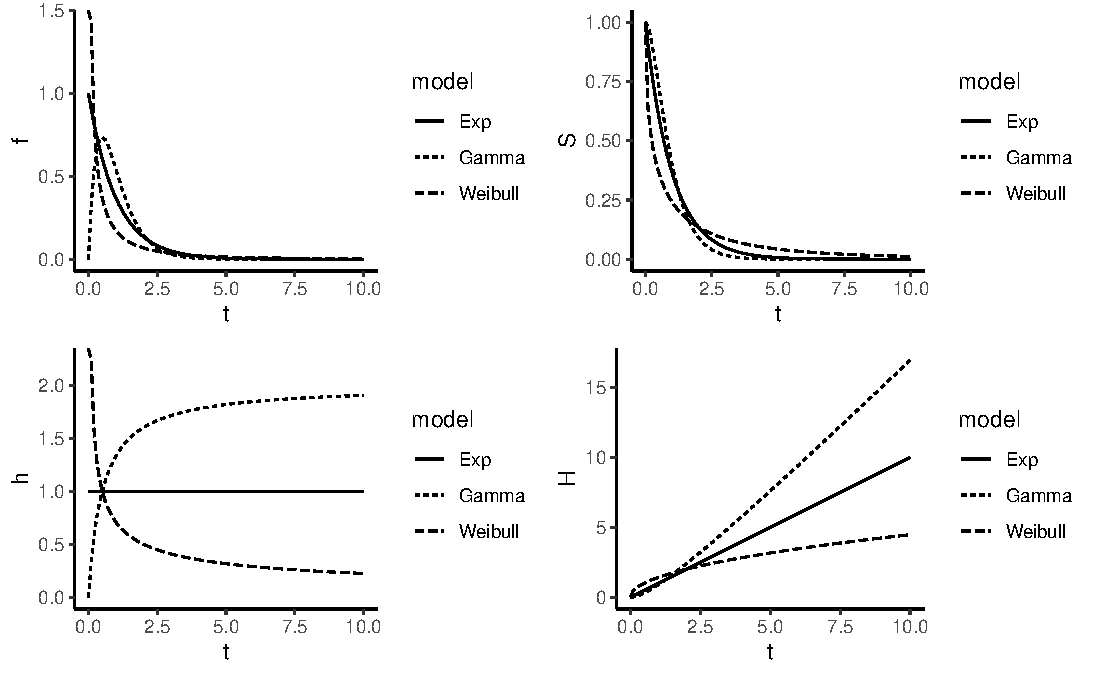
\includegraphics[width = \textwidth]{../figures/d_S_h_H_parametric}
\caption{Fonction de densité, de survie, de hasard et de hasard cumulée des modèles $\ExpDist(\beta = 1)$, $\GammaDist(\alpha = 2, \beta = 1/2)$ et $\WeibullDist(\alpha = 1 / 2, \beta = 1/2)$.}
\label{fig:d_S_h_H_parametric}
\end{figure}
L'approche paramétrique consiste à calibrer plusieurs modèles puis à choisir le plus adapté grâce à des critères d'information.
\subsection{Critère d'information}
Les critères d'informations mesurent l'ajustement du modèle aux données. Ils sont basés sur la vraisemblance et pénalisent la compléxité du modèle (c'est à dire le nombre de paramètres). L'\textit{Akaike Information Criterion} (AIC) est défini par 
$$
\text{AIC} = 2k - 2 l(\Data;\hat{\theta}),
$$
où $k$ désigne le nombre de paramètre du modèle, voir \citet{Akaike1998}. Le Bayesian Information Criteria (BIC) est défini par 
$$
\text{BIC} = k\ln(n) - 2 l(\Data;\hat{\theta}),
$$
où $n$ désigne la taille de l'échantillon voir \citet{Schwarz1978}. le meilleur modèle est caractérisé par la plus petite valeur d'AIC et de BIC. le terme $- 2 l(\Data;\hat{\theta})$ correspond à la déviance du modèle par rapport au modèle qui aurait généré les données. 
\subsection{Test d'adéquation}
Une validation des modèles peut s'effectuer via des test d'adéquation statitique. Les hypothèses du test sont 
$$
\begin{cases}
H_0&\Prob(T\leq t)  = F(t; \theta)\\
H_1&\Prob(T\leq t)  \neq F(t; \theta)
\end{cases}
$$
les statistique de test sont définies par des écarts entre la fonction de répartition du modèle considéré $F(\cdot ; \hat{\theta})$ et la fonction de répartition empirique 
$$
F_n(t) = \frac{1}{n}\sum_{i=1}^n\ind_{t_i\leq t}.
$$
Le test de Kolmogorov-Smirnov s'appuie sur la distance 
$$
D_n = \underset{t\geq 0}{\sup}|F_n(t) - F(t; \theta)|,
$$
estimée concretement par 
$$
D_n=\max(D_-,D_+)
$$
où
$$
D_- =\underset{i = 1,\ldots n}{\max} i/n -F\left(t_{(i)}; \theta\right),\text{ et }D_- =\underset{i = 1,\ldots n}{\max} F\left(t_{(i+1)}; \theta\right) - i/n.
$$ 
On a le résultat de convergence suivant 
\begin{equation}\label{eq:convergence_ks}
\sqrt{n}D_n\overset{}{\rightarrow} K\text{ en loi,}
\end{equation}
où $K$ est une \va de loi de Kolmogorov. La fonction de répartition n'a pas une forme explicite mais cette distribution a été tabulé et encodé dans les logiciel statistiques. Soit $K_{1-\alpha}$ tel que 
$$
\Prob(K>K_{1-\alpha}) = \alpha.
$$ 
On rejette l'hypothèse $H_0$ si 
$$
\sqrt{n}D_n >K_{1-\alpha}.
$$
\begin{definition}
\begin{enumerate}
	\item $\alpha$ est le niveau du test, c'est à dire la probabilité de rejeter l'hypothèse nulle alors qu'elle est vraie
	$$
	\Prob(\sqrt{n}D_n>K_{1-\alpha}|H_0)
	$$
	\item La puissance du test, est la probabilité de rejeter l'hypothèse nulle alors qu'elle est fausse, soit 
	$$
	\beta = \Prob(\sqrt{n}D_n >  K_{1-\alpha}|H_1)
	$$
	\item La p-value est définie par  
	$$
	\text{p-value} = \Prob(K > \sqrt{n}D_n),
	$$
	On rejette l'hypothèse nulle au niveau $5\%$ si $\text{p-value} \leq 0.05$.
\end{enumerate}
\end{definition}
\begin{remark}
Le résultat de convergence \eqref{eq:convergence_ks} n'est pas valide lorsque les paramètre de la distribution doivent être estimés. Des méthodes de Monte Carlo de type bootstrap paramétrique doivent être mis en oeuvre pour déterminé la valeur critique du test (le $K_{1-\alpha}$).
\end{remark}





